% !TEX TS-program = pdflatex
% !TEX encoding = UTF-8 Unicode 
\documentclass[a4paper,11pt,openright,BCOR=15mm]{scrbook}
\usepackage[onehalfspacing]{setspace}    %   
\usepackage[utf8]{inputenc}
\usepackage[portuges,english]{babel}     
%\usepackage[square,numbers]{natbib}
\usepackage[style=numeric,backend=biber,sorting=none]{biblatex}
\usepackage[normalem]{ulem}
\addbibresource{ref.bib} % The filename of the bibliography
\usepackage{graphicx}               
\usepackage[pdftex]{hyperref}
\usepackage[T1]{fontenc}          
\usepackage{pdfpages}         
\usepackage{lettrine}    
\usepackage{booktabs}  
\usepackage{scrhack}   
\usepackage{scrlayer-scrpage}
\usepackage{ulem} % for underline
\usepackage{xcolor}
\definecolor{cinza1}{RGB}{200,200,200}
\definecolor{cinza2}{RGB}{70,70,70}
\usepackage{vhistory}	%% para versoes....
\newcommand\ChapterFont{}      % usar o tipo de letra normal
\newcommand\SectionFont{}
\pagestyle{scrheadings}
\ifoot[]{\raisebox{-32pt}{
\includegraphics[width=0.15\textwidth]{logos/logoisep}}}
\ofoot[]{\raisebox{-22pt}{
\includegraphics[width=0.10\textwidth]{logos/logo_DEI_big_transparente}}}
\cfoot[\pagemark]{\pagemark}
\automark[section]{chapter}
\usepackage{blindtext}   % \texto para demos 
\usepackage{listings}   %  para listagens com diferentes tipos de letra
\usepackage{fancyvrb}  %  para listagens de codigo
\usepackage{listings}
\usepackage{courier}
\usepackage{float}
\lstdefinestyle{yaml}{
	basicstyle=\color{blue}\footnotesize\ttfamily,
	rulecolor=\color{black},
	string=[s]{'}{'},
	stringstyle=\color{blue},
	comment=[l]{:},
	commentstyle=\color{black},
	morecomment=[l]{-},
	breaklines=true,
	frame=single
}


%%%%%%%%%%%%%%%%%%%%%%%%%%%%%%%%%%%%%%%%%%%%%%%%%%%%%%%%%%%%%%%%%%%%%%%%%%%%
\usepackage[mono=false]{libertine}
%%%%%%%%%%%%%%%%%%%%%%%%%%%%%%%%%%%%%%%%%%%%%%%%%%%%%%%%%%%%%%%%%%%%%%%%%%%%%%%%%%%%%%%%%

\begin{document}
	
	\selectlanguage{english}  
	\frontmatter
	
	\titlehead{
\includegraphics[scale=0.2]{figs/logoisep}
		\hfill 
\includegraphics[scale=0.115]{logos/logo_DEI_big_transparente}
	}  
	
	\title{Systematization of Knowledge on Hardening Kubernetes through Native Configurations} 
	\subtitle{LABCIB}
	
	\author{Master in Informatics Engineering - 2024/2025}        
	
	
\publishers
{
	1190830 - Luís Correia\\ 1190974 - Pedro Lemos\\ 1191526 - Pedro Moreira\\ \texttt{Version \vhCurrentVersion, \vhCurrentDate}\\
}         
  
	
	
	
	\date{Porto, \today} 
	
	
	\maketitle   
	
	
	% Start of the revision history table
	\begin{versionhistory}
		\vhEntry{1}{2024-11-15}{Pedro Moreira}{Initial version and structure}  
		\vhEntry{2}{2024-10-17}{...}{Extended description}  

		

	\end{versionhistory}
	
	\cleardoublepage
	

	
	
	
	\tableofcontents
	\addcontentsline{toc}{chapter}{List of Figures}
	\listoffigures
	
	
	
	% \listoftables 
	
	\mainmatter 
	
	%% =================================
	

	%% =================================
	\chapter{Introduction}
	
\textit{[Description, considering the project, of what under individual responsibility]}
	
	%% =================================
	\chapter{Objectives and Scope}

\textit{	[Description, for what under individual responsibility, that inform the goal, the questions related to functional correctness, metrics used and their values, with partial response to questions, and goal achievement analysis. Explicitly mention the tool report(s).]}

	
	%% =================================	
	\chapter{Methodology}
\textit{	[Description, for what under individual responsibility, that inform the goal, the questions related to maintainability, metrics used and their values, with partial response to questions, and goal achievement analysis. Explicitly mention the tool report(s).]}
	
	


\chapter{Background}

\textbf{Kubernetes} is a container orchestration platform that automates the deployment, scaling, and management of containerized applications. Originally developed by Google and now maintained by the Cloud Native Computing Foundation (CNCF), Kubernetes enables IT teams to deploy and manage applications at scale efficiently using containers.


\section{Kubernetes Components}

Kubernetes architecture is based on a distributed system that consists of two primary types of nodes: master nodes and worker nodes. Each type plays a specific role in ensuring the cluster operates effectively \cite{the_linux_foundation_kubernetes_2024}.

\subsubsection{Master Nodes}\label{sect:masters}
Master nodes are the control center of a Kubernetes cluster. They manage the cluster’s state, handle scheduling, and coordinate operations. The key components running on master nodes are:

\begin{itemize}
	\item \textbf{API Server} (\texttt{kube-apiserver}): Exposes the Kubernetes API and serves as the entry point for all cluster interactions.
	\item \textbf{Controller Manager} (\texttt{kube-controller-manager}): Manages controllers that monitor the clusters state and make adjustments to achieve the desired state.
	\item \textbf{Scheduler} (\texttt{kube-scheduler}): Component that watches for newly Pods without assigned nodes, and selects one for them to run on. Some factors are taken into the decision, like hardware/software/policy constraints, data location, deadlines, among others.
	\item \textbf{etcd}: Stores all configuration data and the state of the cluster in a consistent and reliable way.
	\item \textbf{Cloud Controller Manager} (\texttt{cloud-controller-manager}): This component runs cloud-provider-specific controllers that manage resources outside the Kubernetes cluster. It is only active when the cluster is hosted on a cloud platform.
\end{itemize}

\subsubsection{Worker Nodes}

The main responsibilities of a worker node is to process data stored within the cluster and managing networking to ensure seamless communication both between applications within the cluster and with external systems. The control plane assigns tasks to the worker node to carry out these functions. The key components are:

\begin{itemize}
	\item \textbf{Kubelet}: An agent that ensures containers are running and in healthy state according to specifications.
	\item \textbf{Kube Proxy}: Manages network routing and load balancing at the network level.
	\item \textbf{Container Runtime}: The software responsible for running containers.
\end{itemize}

\section{What is etcd?}

etcd is a distributed key-value database essential for storing the cluster’s state and configuration. It ensures data consistency across all nodes using the Raft consensus algorithm, which keeps all nodes in sync even during failures, providing a reliable foundation for Kubernetes operations \cite{etcd_faq_2024}.

A leader is elected among the etcd nodes to manage all write operations, while follower nodes stay synchronized with the leader. If the leader fails, the Raft algorithm ensures a new one is elected quickly, maintaining high availability and preventing service disruption \cite{etcd_faq_2024}.

Additionally, etcd persistently stores the cluster's state, allowing Kubernetes to retrieve and update this information in real-time. It holds metadata and operational data for Kubernetes objects like pods, deployments, and services, enabling the Kubernetes API server to query etcd and consistently enforce the cluster’s desired state \cite{etcd_faq_2024}.

\section{What are Kubernetes Secrets?}

\textbf{Secrets} are objects used to store sensitive data, such as passwords, API tokens, or SSH keys. Instead of embedding this information directly into code or configuration files, Secrets allow secure storage and controlled access to sensitive information \cite{the_linux_foundation_secrets_2024}.

\subsection{Key Features of Secrets}
\begin{itemize}
	\item \textbf{Storage}: Secrets are base64 encoded before being stored in \texttt{etcd}, but not encrypted by default. Kubernetes can be configured to encrypt them at rest using tools like Key Management Service (KMS).
	\item \textbf{Usage}: Secrets can be mounted as volumes in containers or passed as environment variables, which allows secure handling of credentials.
\end{itemize}
		
	%% =================================		
\chapter{Kubernetes Native Configurations for Hardening}
Having introduced what Kubernetes is, we are now able to delve into the main purpose of this report, which is to systematize what built-in features and configurations of this technology we can use to improve a cluster's security posture and resistance to cyber-attacks.
This chapter will be split into various sections, each concerning an area of relevance when it comes to Kubernetes Hardening. In each section, a context regarding the security improvements that are available will be presented, and consequently the measures through which one can implement these improvements will also be showcased.

	\section{Data Encryption}\label{sect:data}
	
As we've seen in the context section of this report, Kubernetes stores Secrets and their data on the etcd backend database without any form of encryption \cite{the_linux_foundation_secrets_2024} - despite encoding them with Base64, which does not constitute encryption as the plain-text contents are directly obtainable. If an attacker is able to access either the API server or the etcd database directly, he will be able to obtain the plain-text contents of the secrets that are managed by that cluster. One can easily picture the compromise that this can cause, as secrets usually contain business-critical credentials that are used by services running in Kubernetes. For instance, an application Pod might need to access a database, and thus read the connection string and database user credentials from a secret. If an attacker could obtain the content of this secret, he too would at least have the credentials to access the database.

Fortunately, Kubernetes provides a series of configurations that can be applied to encrypt Secrets - and other resources - at rest. This is done through the configuration of some resources on the cluster's API server. Notably, Kubernetes defines the \texttt{EncryptionConfiguration} Custom Defined Resource (CRD), which allows practitioners to customize what resources shall be encrypted and through what mechanism (also known as provider) \cite{the_linux_foundation_encrypting_2024}.

The flow of actions is as follows: a user or application creates a Secret by sending an API call to the Kubernetes API; the API checks its \texttt{EncryptionConfiguration} file to evaluate what encryption provider to use and which key to use for that provider; if a provider is specified, as well as the key to use, the API server uses both to encrypt the provided data; then, this encrypted data is stored in etcd. For the decryption, the API retrieves the secret from etcd and uses the aforementioned \texttt{EncryptionConfiguration} to decrypt the contents.

In \ref{code:encConfig}, we present a simple example of an \texttt{EncryptionConfiguration}. What this does is instruct the Kubernetes API that all Secrets must be encrypted using the \texttt{aescbc} provider, using the encryption key specified in \texttt{keys.secret} field.


\begin{lstlisting}[style=yaml,caption={EncryptionConfig example},label=code:encConfig]
	apiVersion: apiserver.config.k8s.io/v1
	kind: EncryptionConfiguration
	resources:
	- secrets
	providers:
	- aescbc:
	  keys:
	    - name: key1
	      secret: <BASE 64 ENCODED SECRET>
	- identity: {}
\end{lstlisting}

There are several providers which we can use when encrypting secrets, which are specified in the Kubernetes documentation itself \footnote{This comparison can be seen in \href{https://kubernetes.io/docs/tasks/administer-cluster/encrypt-data/\#providers}{\underline{this documentation link}}}. Some facts are worth noting:

\begin{itemize}
	\item The \texttt{identity} provider does not encrypt data. It's the default used by Kubernetes, as we've covered before. Despite this, it has practical utilities, such as serving as one of the encryption providers for instance when migrating clear-text secrets to encrypted ones. So, despite not encrypting data, it would be improper to discard its existence;
	\item The \texttt{aescbc}, \texttt{aesgcm} and \texttt{secretbox} providers require the encryption key to be specified in the encryption configuration file. Using them protects a cluster in the event of a compromise, but if the hosts in which the Kubernetes API is running are themselves compromised, this does not provide additional security, as the attacker will be able to obtain the encryption key from the local filesystem \cite{gkatziouras_kubernetes_2024}. Nonetheless, it's an improvement from the default configuration.
\end{itemize}

Besides the providers mentioned above, there exists the \texttt{kms} provider, which is currently in version 2 - and version 1 is deprecated. This provider offers a more complex - but more secure - encryption solution. It's purpose is to solve the issue of having the encryption key defined in a local file, as we've covered previously. To address this matter, the kms provider calls upon two new components \cite{gkatziouras_kubernetes_2024}: 

\begin{itemize}
	\item An external Key Management Service (KMS);
	\item A Kubernetes KMS provider plugin, which is responsible for connecting with the external KMS for the encryption and decryption processes.
\end{itemize}

This mechanism adopts an "envelope encryption scheme using a two-key approach" \cite{gkatziouras_kubernetes_2024}, with those keys being: the Data Encryption Key (DEK), which is used to encrypt the resources referenced in the \texttt{EncryptionConfig}; and the Key Encryption Key (KEK), which is used to encrypt the DEK and is hosted remotely on the KMS. This way, having the encryption key on a separate system, the main downside of the previous solutions is addressed, since a filesystem compromise of the Kubernetes master nodes wouldn't directly lead to a compromise of the secrets stored in the cluster.

However, we must note that the usage of the \texttt{kms} provider requires the usage of third-party tooling, not native to Kubernetes - since it requires the usage of an external KMS. 

% pensar se vale a pena mencionar o Trousseau/kleidi (https://beezy.dev/kleidi/#) e o Hashicorp Vault a servir como KMS

	\section{API Server Configurations}
	
The API server is an essential component of Kubernetes, as we've explained in \ref{sect:masters}. It is responsible for handling all administrative operations and communications within the cluster, and thus acts as the primary interface for practitioners to interact with the Kubernetes environment. Given its critical role, the API Server is a frequent target for attackers aiming to exploit vulnerabilities, gain unauthorized access, or disrupt cluster operations.

Securing the API server is, thus, a crucial task that cluster administrators must undergo to ensure the integrity, confidentiality and availability of this environment. Misconfigurations or weak security settings can expose the cluster to numerous risks, such as unauthorized access to data, or disruption of operations.

Therefore, to assist practitioners in undergoing this process, we will look into relevant API server configurations which will improve its security posture.

Before proceeding, it's important to note that the API server can be interacted with through many means, such as the \texttt{kubectl} utility, as well as REST requests. This highlights the relevance of appropriate firewall practices. Access to the Kubernetes API must be properly limited to business-related needs. A good approach for this is to allow only an organizational VPN's IP or set of IP addresses to make requests to the API, thus limiting the attack vectors. However, were this firewall or VPN to be compromised, further security measures are necessary.

\subsection{Authentication}
\label{subsec:auth}

When a user attempts to interact with the API server, he must first undergo a process of authentication. This verifies the identity of a user or service before allowing them to communicate with the API server. Kubernetes supports multiple authentication methods which can be employed \cite{the_linux_foundation_authenticating_2024}.

\subsubsection{X.509 Client Certificates}

Kubernetes is able to use certificates for authentication purposes. For this effect, the API server must be started with the \texttt{--client-ca-file} flag which should point towards one or more valid Certificate Authority (CA) files, which will be used to validate the certificates used by clients when issuing requests to the API \cite{the_linux_foundation_authenticating_2024}. These certificates can be generated manually using tools such as \texttt{easyrsa} and \texttt{openssl}.

With this method "any user that presents a valid certificate signed by the cluster's certificate authority (CA) is considered authenticated" \cite{the_linux_foundation_authenticating_2024}. A more proper way to use this is to have users generate their own private key, as well as a Certificate Signing Request (CSR) which specifies necessary attributes that a user certificate must have. Notably, the subject of the certificate will be used by Kubernetes to identify the username of a client, and thus using it for authorization purposes. Then, this CSR is validated and signed by the administrator, using the CA of the cluster, and the certificate is distributed to the client.

This ensures that each user has an account, and further ensures traceability and accountability of any user's actions. However, the manual distribution of certificates might be a hindrance on organizations which are larger and more complex. Nonetheless, it's a native setting of Kubernetes that ensures the hardening of the authentication process. 

\subsubsection{Service Account Token}

These are signed JSON Web Tokens (JWT) which Kubernetes generates so that entities can communicate with the API server \cite{the_linux_foundation_authenticating_2024}. These tokens are associated with ServiceAccount objects, which by default represent the identity of an application in Kubernetes \cite{martin_hacking_2021} - their function will be expanded upon in the RBAC section. It's unusual that these tokens are used for the authentication of users, as they are more frequently used by Pods which require to communicate with the Kubernetes API, or by processes that run outside of the cluster but frequently need to talk with its API.

\subsubsection{OpenID Connect (OIDC)}

This authentication mechanism relies on a third-party identity provider, such as Google or Keycloak, for the generation of a JWT which the user can then present to the API server in order to issue requests \cite{the_linux_foundation_authenticating_2024}. It's still relevant in the scope of this Systematization of Knowledge, as even though it resorts to an external mechanism, it uses a configuration that's available in Kubernetes itself.

It's worth noting that, unlike workloads - which are represented in Kubernetes via Service Accounts - human users are not represented by Kubernetes objects \cite{the_linux_foundation_authenticating_2024,martin_hacking_2021}. Therefore, integrating with an external source-of-truth for users such as the ones mentioned above is optimal for handling user interaction with the API Server. The applicability of this can be easier when using a cloud instance, as practitioners can check what options their cloud provider offers \cite{martin_hacking_2021}, but technologies like Keycloak or Dex enable organizations to deploy an identity management system on their own infrastructure.

\subsubsection{Webhook Token Authentication}

Users are able to specify authentication tokens on their requests to the API, which must contain the value of this token on the Authorization header of the request. What this authentication method relates to is the assessment of the validity of the provided token.

It works by using a remote webhook service when determining user privileges \cite{the_linux_foundation_webhook_2024}. This external service responds to REST requests and allows or denies access to the requested resources. It's essentially a way to delegate the authorization process to a third-party, thus allowing administrators to inject their custom logic as part of an authorization policy \cite{eknert_kubernetes_2022}.

\subsubsection{Anonymous Requests}

Besides these login mechanisms, there is the concept of anonymous requests. When enabled, "requests that are not rejected by other configured authentication methods are treated as anonymous requests" \cite{the_linux_foundation_authenticating_2024}. As such, a user would be able to query the API without identifying himself which, if proper RBAC configurations are not employed, could be quite damming to an organization. As such, it is advised that anonymous requests are disabled by using the \texttt{--anonymous-auth=false} on the API server. If it needs to be enabled due to organizational needs, it's paramount to ensure that the permissions of unauthenticated users are as restrictive as possible.

\subsection{Admission Controllers}

%Explicar o flow do Kubernetes, primeiro autenticaçao, depois autorizaçao (que vem do RBAC ou ABAC), e finalmente admission (podemos usar esta imagem https://kubernetes.io/docs/concepts/security/controlling-access/).
%
%
%validating ou mutating, falar disso e da diferença
%
%Admission controllers do not (and cannot) block requests to read (get, watch or list) objects. -> importante realçar isto, referir que os requests nao cobertos por admission control devem ser cobertos por RBAC e gestao de permissoes
%
%https://kubernetes.io/docs/reference/access-authn-authz/admission-controllers/
%https://kubernetes.io/blog/2022/01/19/secure-your-admission-controllers-and-webhooks/
%https://kubernetes.io/docs/concepts/security/controlling-access/\#admission-control
%
%os default sao: CertificateApproval, CertificateSigning, CertificateSubjectRestriction, DefaultIngressClass, DefaultStorageClass, DefaultTolerationSeconds, LimitRanger, MutatingAdmissionWebhook, NamespaceLifecycle, PersistentVolumeClaimResize, PodSecurity, Priority, ResourceQuota, RuntimeClass, ServiceAccount, StorageObjectInUseProtection, TaintNodesByCondition, ValidatingAdmissionPolicy, ValidatingAdmissionWebhook
%
%configurar o EventRateLimit pode ser interessante para evitar algum tipo de flood de eventos que um atacante pudesse causar?
%
%falar de configurar as ResourceQuotas em cada deployment talvez?

When considering interactions with the Kubernetes API, there are three actions that take place: authentication, authorization, and admission. This is clearly illustrated in Figure \ref{fig:authflow}. It's worth highlighting that both human users, as well as Pods, go through the same access control flow, further showcasing the versatility of Kubernetes authentication and authorization methods.

\begin{figure}[h!]
	\centering
	\label{fig:authflow}
	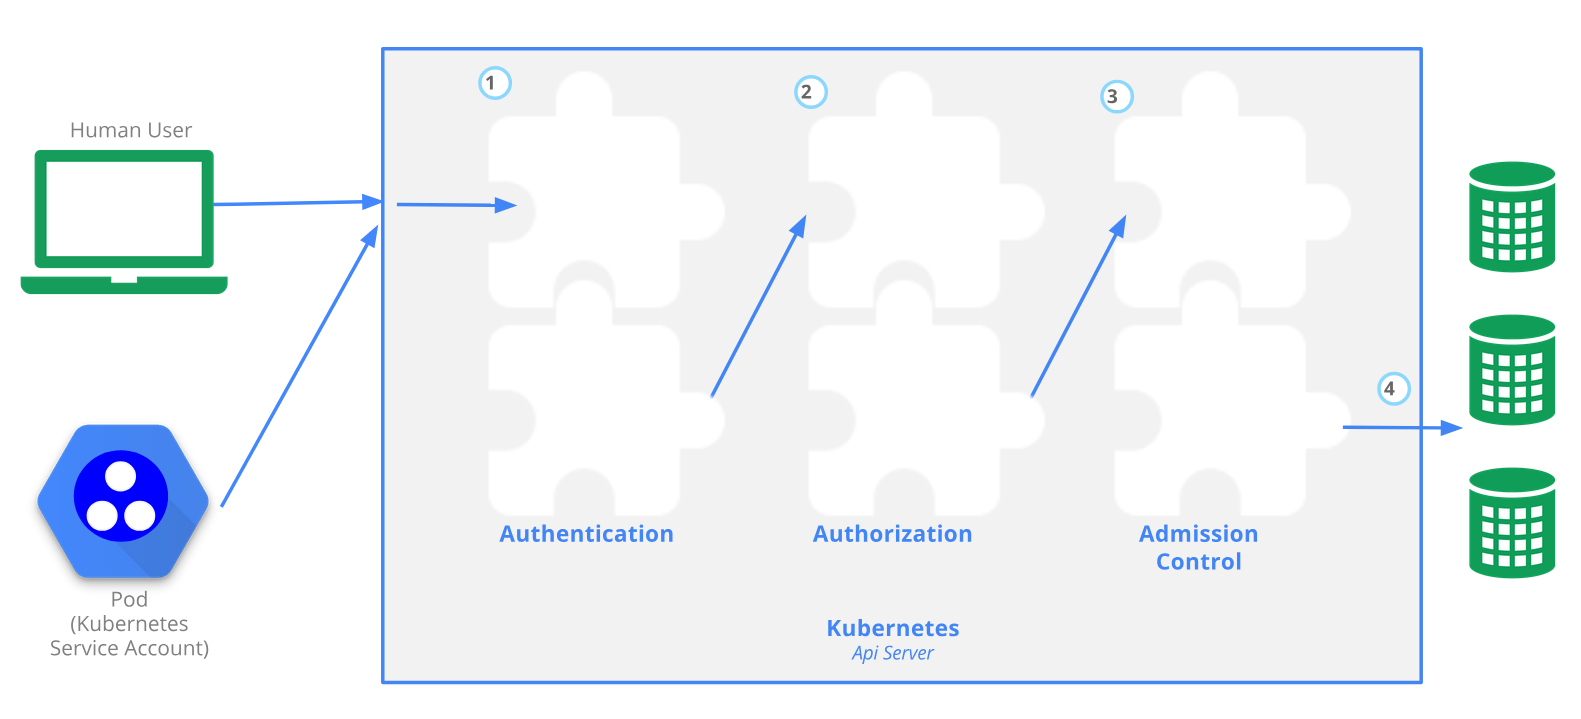
\includegraphics[scale=0.3]{figs/access-control-overview.png}
	\caption{Access Control Overview \cite{the_linux_foundation_controlling_2023}}
\end{figure}


The first one has been explored in \ref{subsec:auth}, covering the different methods supported by Kubernetes, as well as recommendations. Considering authorization, this will be covered in \ref{sec:auth}. So, we must now cover the admission phase, as it's the last in the process, as well as a crucial part of it.

In Kubernetes, the admission process is handled by Admission Controllers. These are "software modules that can modify or reject requests" \cite{the_linux_foundation_controlling_2023}. They do so by intercepting requests to the API before the persistence of resources \cite{the_linux_foundation_admission_2024}. Note that the persistence of resources is being specifically mentioned, excluding other types of operations. This is because admission controllers only operate on "requests that create, delete, or modify objects" \cite{the_linux_foundation_admission_2024}. As such, read operations (the \texttt{get}, \texttt{watch} or \texttt{list} verbs) must be strictly covered by RBAC policies.

Admission controllers may be validating, mutating, or both. With validating admission controllers, the resources are validated against the set of modules to ensure that they comply with the rules imposed by them, and are only persisted in the cluster if they pass all controllers. In the case of mutating controllers, however, they may modify the data for the resource that's being modified \cite{the_linux_foundation_admission_2024}.

These modules are enabled at the API level, as we've seen. This is done by using the \texttt{--enable-admission-plugins} flag with the controllers that we want to enable. As such, to see what admission controllers are currently enabled in the cluster, we can investigate the manifest of the Pod that runs the API server in the cluster. An example of this is showcased in Figure \ref{fig:admission}.

\begin{figure}[h!]
	\centering
	\label{fig:admission}
	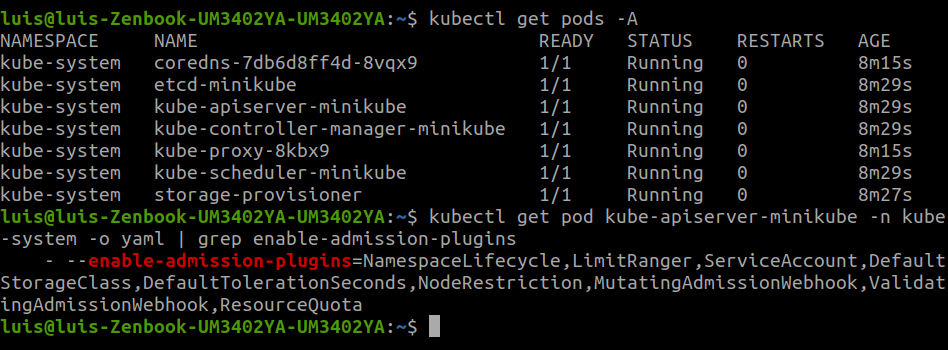
\includegraphics[scale=0.5]{figs/enabled-admission.png}
	\caption{Enabled admission controllers in testing instance}
\end{figure}

By consulting the Kubernetes documentation in \cite{the_linux_foundation_admission_2024}, we're able to confirm that the default admission controllers in version 1.31 are the ones shown in \ref{code:admission}.

\begin{lstlisting}[style=yaml,caption={Default Admission Controllers},label=code:admission]
	CertificateApproval, CertificateSigning, CertificateSubjectRestriction, DefaultIngressClass, DefaultStorageClass, DefaultTolerationSeconds, LimitRanger, MutatingAdmissionWebhook, NamespaceLifecycle, PersistentVolumeClaimResize, PodSecurity, Priority, ResourceQuota, RuntimeClass, ServiceAccount, StorageObjectInUseProtection, TaintNodesByCondition, ValidatingAdmissionPolicy, ValidatingAdmissionWebhook
\end{lstlisting}

Thus, we're able to confirm that our testing instance is missing some of the defaults, which should be enabled. To enable them, we can simply edit the \texttt{kube-apiserver} manifest, adding the necessary controllers to the flag shown in Figure \ref{fig:admission}.

The available Admission Controller plugins vary vastly in functionality, and cover the validation and mutation of requests "mostly from the resource management and security points of view" \cite{sayfan_mastering_2020}. Our recommendation is for practitioners to:

\begin{enumerate}
	\item Validate what Admission Controllers are currently enabled in the cluster;
	\item Investigate what plugins can be useful in their specific organizational context. This can be done by consulting the documentation of each controller's function \footnote{Presented in \href{https://kubernetes.io/docs/reference/access-authn-authz/admission-controllers/\#what-does-each-admission-controller-do}{\underline{this documentation link}}}, and evaluating if it responds to any organizational needs.
\end{enumerate}

Besides these recommendations, we must also consider the ResourceQuota and LimitRanges admission controllers separately, as their implementation is quite helpful in ensuring the proper deployment of applications in a Kubernetes cluster.

\subsubsection{ResourceQuotas and LimitRanges}

Kubernetes offers the ResourceQuota and LimitRanges admission controllers by default, which can be used to restrict resource usage for namespaces, nodes or Pods \cite{national_security_agency_kubernetes_2022}.

Resource quotas can be used to limit the aggregate resource consumption per namespace \cite{the_linux_foundation_resource_2024}. With them, practitioners can manage their computational resources used by their clusters' namespaces more effectively. For instance, they can be used to limit the total amount of CPU and memory requested and/or used by each namespace.

It's worth noting the difference between the requested and the used values, as an administrator must be aware of this to properly define the resource quotas for the cluster. Considering the CPU and memory attributes, the requested value represents the resources the Pod specifies at the time of its initialization. This does not mean that the Pod will automatically use the requested amount of CPU and memory, but that it will require them during the execution. As an example, a Pod can request 1Gi of RAM, but only consume 100Mi while it's executing. However, if the memory usage has any spike during the Pod's operation - for instance, due to a spike in traffic - it will be able to use more of it, since that initial request has been allocated to it.

Further analyzing this example scenario, if this memory spike were to increase further, it could hinder the operation of the cluster as a whole, since it's exhausting the resources. This is where the concept of limits is useful. If a limit of memory is defined in this case, the pod will be able to use more that it has requested - as we've explained prior - but not more than the defined limit.

Having this context established, we assert as a good practice to define resource quotas which impose maximum values not only on the compute power requested for a namespace, but also on the limits which said namespace will not be able to exceed. A practical example of a ResourceQuota manifest matching this description is presented in \ref{code:reqquota}.

\begin{lstlisting}[style=yaml,caption={ResourceQuota example},label=code:reqquota]
	apiVersion: v1
	kind: ResourceQuota
	metadata:
	  name: example-cpu-mem-resourcequota
	spec:
	  hard:
	    requests.cpu: "1"
		requests.memory: 1Gi
		limits.cpu: "2"
		limits.memory: 2Gi
\end{lstlisting}


Whereas a ResourceQuota imposes a limit on the resources used by a namespace, the LimitRange policy imposes limits per Pod \cite{national_security_agency_kubernetes_2022}. It's objective is to help adminstrators ensure "that a single object cannot monopolize all available resources within a namespace" \cite{the_linux_foundation_limit_2024}. As such, it provides constraints to limit resource allocations per Pod or even container within each Pod, as well as storage requests per each \texttt{PersistentVolumeClaim}. In \ref{code:limitrange}, we present an example of a LimitRange manifest which could be applied in a cluster.


\begin{lstlisting}[style=yaml,caption={ResourceQuota example},label=code:limitrange]
apiVersion: v1
kind: LimitRange
metadata:
  name: cpu-resource-constraint
  namespace: demo
spec:
limits:
- default:
    cpu: 500m
  defaultRequest:
    cpu: 500m
  max:
    cpu: "1"
  min:
    cpu: 100m
  type: Container
\end{lstlisting}

What the presented manifest does is:
\begin{enumerate}
	\item Define the default CPU limit and request for containers in the "demo" namespace as 500m. What this means is that, if no request or limit is specified in the Pod, it will be set to 500m;
	\item Define that the maximum CPU a container can request is 1;
	\item Define that the minimum CPU a container can request is 100m.
\end{enumerate}

It's important to note that the LimitRange admission controller "does not check the consistency of the default values it applies" \cite{the_linux_foundation_limit_2024}. This means that the values which are applied could generate a conflict with the container that's being started. For instance, and still considering the LimitRange in \ref{code:limitrange}, if we were to start a Pod that specifies a container which requests 700m of CPU, this policy wouldn't alter this request, but would set the limit to 500m. Thus, the Pod wouldn't be scheduled, since the request can never be bigger than the limit.

We advise cluster administrators to set \texttt{ResourceQuotas} and \texttt{LimitRanges} according to the needs of their applications. While not strictly a security concern, it could mitigate potential issues in the cluster, which could originate some exposure to attacks.

\subsection{API Server Security Flags}



%(https://chatgpt.com/share/674613c5-f8c8-8013-80ee-268d0270a2e1)
%
%List and explain important API Server flags for hardening the cluster:
%
%a. Network Security
%
%
%--tls-cert-file and --tls-private-key-file:
%Configure TLS to encrypt communication.
%
%--enable-bootstrap-token-auth=true:
%Use temporary tokens for secure cluster bootstrapping.
%
%c. Audit Logging
%
%--audit-log-path and --audit-log-maxage:
%Enable and configure audit logs to track all API requests and detect malicious activity.
%


Throughout this chapter, we've already explored some API configurations that can be enabled to harden the security posture of a Kubernetes cluster. Besides those, there are several others which we find relevant to systematize in the present document. That is, therefore, the goal that this subsection aims to achieve.


In 2020, the vulnerability CVE-2020-8558 \cite{national_institute_of_standards_and_technology_nvd_2020} was reported. It states that there was a defect in the kubelet and kube-proxy components which allowed attackers on the local network of the cluster, or in malicious pods with specific capabilities running in it, to exploit the API server. This was because they were able to access services bound to the localhost address from the local network, which should not be possible. This highlighted the importance of ensuring that the flag \texttt{--secure-port} is configured, so that the API listens on a secure port \cite{the_linux_foundation_kube-apiserver_2024}.

Also related to the \texttt{--secure-port} flag, we advise administrators to also set the \texttt{--bind-address} configuration, which sets the IP address on which the API will listen to for requests \cite{the_linux_foundation_kube-apiserver_2024}. This should be set to an address on the local network, ensuring that the API is not exposed on a server's public IP. Keep in mind that, if this is implemented, a VPN or reverse proxy will be required for administrators to communicate with the API.

The Kubernetes API also allows administrators to configure audit policies \cite{the_linux_foundation_auditing_2024}. These record "the chronological set of records documenting the sequence of actions in a cluster" \cite{the_linux_foundation_auditing_2024}, logging activities that are performed by users, by applications that interact with the API, and by the control plane itself. Similarly to the \texttt{EncryptionConfiguration} shown in \ref{sect:data}, this feature requires the definition of a manifest, which is then referenced on the Kubernetes API configuration. In \ref{code:auditpol}, we present an example audit policy, which we'll explore.

\begin{lstlisting}[style=yaml,caption={ResourceQuota example},label=code:auditpol]
	apiVersion: audit.k8s.io/v1
	kind: Policy
	rules:
	  - level: Metadata
	    verbs: ["create"]
	    namespaces: ["demo"] 
	    resources:
	      - group: ""   
	    resources: ["pods"]
	
	  - level: RequestResponse 
	    resources:
	      - group: ""
	        resources: ["namespaces"]
\end{lstlisting}

In this example, we're logging two types of activities:
\begin{enumerate}
	\item All creations of Pods in the "demo" namespace;
	\item All activities related to namespaces in the cluster, including creation and deletion.
\end{enumerate}

We can also see different values in the "level" key of each entry in the "rules" list. There are four possible values \cite{the_linux_foundation_auditing_2024}:
\begin{itemize}
	\item None: Does not log the events that match the rule;
	\item Metadata: Logs the event that matches the rule with the respective metadata, but doesn't include the request or response body;
	\item Request: Logs the events with request metadata and body, but does not log the response body;
	\item RequestResponse: Logs events with the request and response's metadata and body.
\end{itemize}

So, for the creation of namespaces, the policy in \ref{code:auditpol} will log both the request and response's metadata and body, whereas for the creation of pods, only the metadata will be recorded.

Now that the \texttt{Policy} manifest has been created, it must be referenced in the API configuration so that it can be used by the cluster. This is done by using the \texttt{audit-policy-file} and \texttt{audit-log-path} fields when configuring the API, as shown in Figure \ref{fig:auditconf}. Bear in mind that, for this example, we're outputting the logs to the standard output, which is the logs of the \texttt{kube-apiserver} pod.

\begin{figure}[h!]
	\centering
	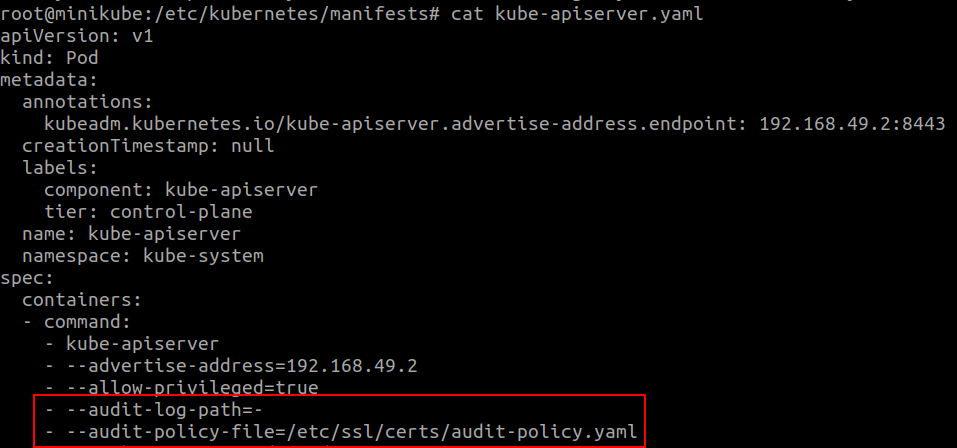
\includegraphics[scale=0.5]{figs/api-config-audit.png}
	\caption{Configuration of API server for audit logs}
	\label{fig:auditconf}
\end{figure}

As an example, Figure \ref{fig:audit-namespace} demonstrates the audit log of a response to a request which creates the "demo" namespace.

\begin{figure}[h!]
	\centering
	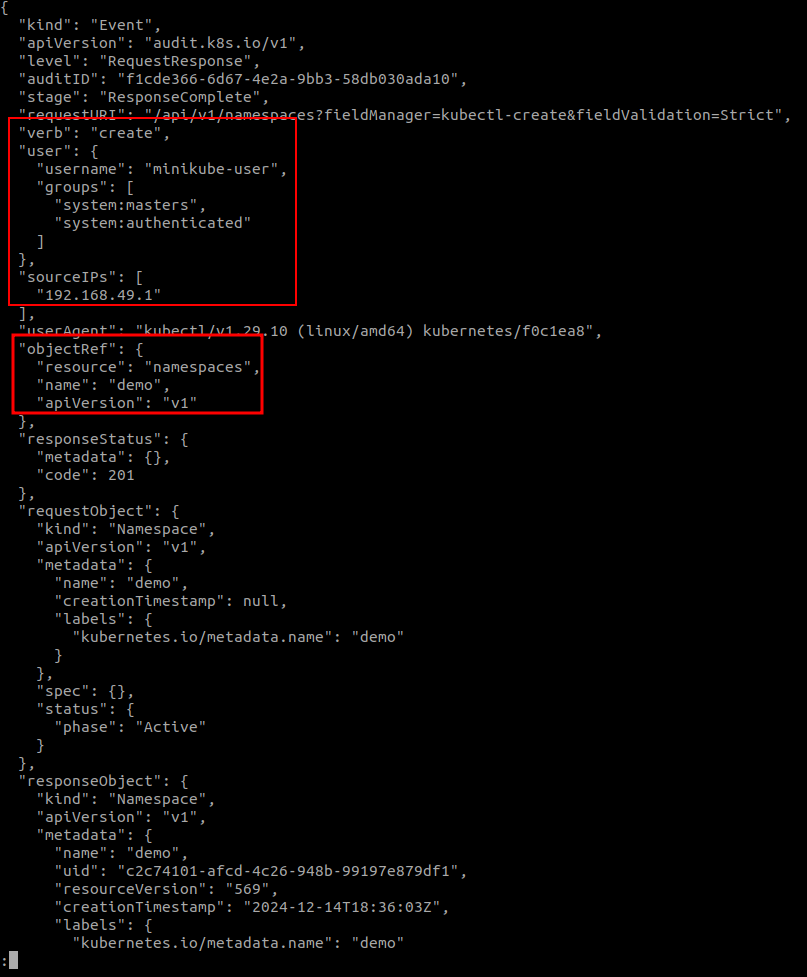
\includegraphics[scale=0.4]{figs/audit-namespace-create.png}
	\caption{Audit logs of a namespace creation}
	\label{fig:audit-namespace}
\end{figure}

In these logs, we can see some very useful information, such as the IP address from where the request originated, the username of who performed it and their RBAC groups. However, we can also infer that logging events with the \texttt{RequestReponse} level might not be appropriate for every case, as there's a lot of information to go through. For comparison, we present a \textit{Metadata}-level log of a pod created in the "demo" namespace - matching the audit rule - in Figure \ref{fig:audit-pod}.

\begin{figure}[h!]
	\centering
	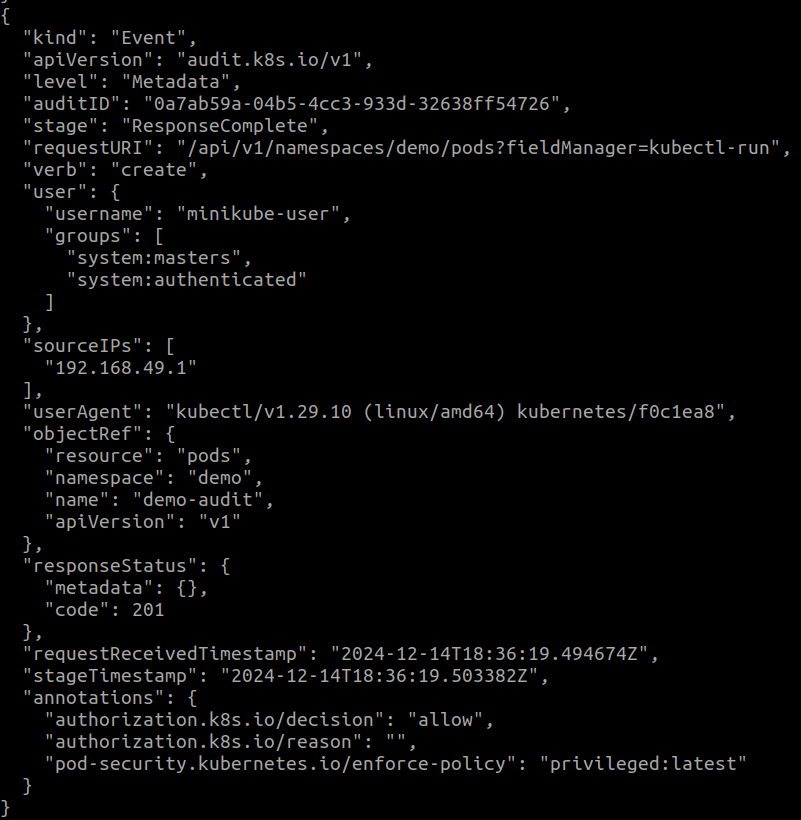
\includegraphics[scale=0.4]{figs/audit-pod-create.png}
	\caption{Audit logs of a pod creation}
	\label{fig:audit-pod}
\end{figure}

From this log, we can clearly extract that the \texttt{demo-audit} pod was successfully created in the \texttt{demo} namespace - due to the 201 response code. We can also see exactly when it was created, and by what user and IP address.

The importance of these audit policies now becomes clear, as the data contained within them can assist practitioners in keeping track of the actions that take place in the cluster. Another factor which adds to the usability of this feature is the configurable granularity of the logs that are captured. With this, administrators can fine-tune audit policies based on their organizational requirements, thus ensuring that relevant actions are captured with the necessary detail.

	\section{Network Policies}
	
	\section{RBAC and Authentication}
	\label{sec:auth}
		
	%% =================================
\chapter{Complementary Tooling}

While Kubernetes provides robust built-in capabilities for container orchestration, there is a broad list of complementary tools that allow to extend these capabilities.  These tools enhance areas such as advanced security features and comprehensive monitoring to strengthen cluster security. This section highlights several tools that offer security-enhancing features and explains how each contributes to improving cluster security.

\section{Network and Security}\label{sect:complementNetSec}
Text, text, text...

\section{RBAC}\label{sect:complmentRbac}
Text, text, text...

\section{Monitoring and Logging}\label{sect:complementMonitor}
Text, text, text...

	%% =================================
	\chapter{Analysis and Best Practices}
 \textit{	[Description, for what under individual responsibility, that inform the goal, the questions related to architectural compliance, metrics used and their values, with partial response to questions, and goal achievement analysis. Explicitly mention the tool report(s).]}
	


	%% =================================
	\chapter{Conclusions }
 ...\newline



%	
%	\bibliographystyle{ACM-Reference-Format}
%	\renewcommand\bibname{References}
%	\bibliography{ref}
%	\label{references}
%	\addcontentsline{toc}{chapter}{References}
	
	\printbibliography[heading=bibintoc]
	
	
\end{document}